\chapter{Method}\label{cha:Method}

% längsta avsnittet i rapporten. Den består av en redogörelse av ditt arbete och den visar hur du kommer fram till dina resultat.

% Undvik egna synpunkter. Dessa framförs i Inledningskapitlet och Diskussions-kapitlet

% Ange källa till figurer i slutet. T.ex.  Source: Expedition Mondial.

% Metoddelen beskriver tillvägagångssättet – intervjuer, observationer, litteraturstudier, laborationer och så vidare. Motivera varför en viss metod valdes och vilka eventuella svårigheter som har förekommit. Metoden ska vara replikerbar, vilket innebär att en annan skribent ska kunna göra om studien med hjälp av informationen i metoddelen. Det finns en mängd böcker om olika vetenskapliga metoder. Till exempel kan en intervju utföras på en mängd olika sätt. I rapporter inom humaniora brukar metoddelen vara mer utförlig än i en teknisk rapport.

Using novel methods like \textit{service design} when developing the app according to research question \#1 and \textit{data-driven design} and interviews for understanding interaction according to research question \#2.

%\section{Preparations in Sweden}

These were the insights before going to Uganda, addressed in the initial work plan.

\section{Answering research questions \#1}

\textbf{\textit{How the topic of Entrepreneurship affects the work}}\\
The scope of the app is to examine the entrepreneurship the student already has. The goal is to give good feedback.

Entrepreneurship is a developing area of research. The topic and the YoungDrive's methology largely effects the work, via its ethos "Dream big, start small", "Can you sell?", and emphasis on fun. Their existing training material and the structure of the program needs to be taken in consideration.

Entrepreneurship means using a learning by doing methodology. A challenging part of the work is that YoungDrive consists of both the practical skills of the entrepreneur, theoretical material of running a business, and an entrepreneurial mindset. Therefore, both how to assess knowledge, and build habits, needs to be examined.

\textbf{\textit{How a Physical education affects the work}}\\
The physical vs. digital interplay needs to be closely examined. How does the app interplay with the physical education? For this, service design methodology will be used. \\

\textbf{\textit{How the Time Constraints and Cultural Differences affects the work}}\\

The biggest challenge with regards to time constraints and cultural differences is that it is difficult to understand the audience.\\

Action:
\begin{itemize}
    \item It led to me started planning the master thesis several months ago
    \item It led to me choosing to spend 3 months in Uganda, because the client and academy is there, and start the design process when I'm there
    \item It led me to the topic of Service Design
\end{itemize}

Positives:
\begin{itemize}
    \item I will come closer to the client and coaches by moving to Uganda, which is necessary when taking a service design approach
\end{itemize}

Negatives:
\begin{itemize}
    \item I will have limited internet outside of the work location
    \item Long distances between work place and home compared to Sweden
    \item I will still have long distances and limited access to coaches\\
\end{itemize}

These negatives needs to be overcome, by narrowing down the scope of the thesis work. \\

\textbf{\textit{How the Design Constraints affects the design process}}\\
"Simple" in this cultural setting leads to design constraints and that design methodology becomes very important.\\

\textbf{\textit{How the Technical Constraints affects the technologies used}}\\
Limitations on internet/electricity means:

\begin{itemize}
    \item Web app
    \item Localized
    \item Database
    \item Fetch/pull functionality in the app
    \item Battery preserving app needed
\end{itemize}

Also, me as a developer have limited experience of building apps, and time constraints. As such, technical compromises should be made.

Furthermore, existing tools could be used, instead of building the app from scratch. E.g. using existing tools like Knowly or Typeform\footnote{examples include https://showroom.typeform.com/to/ggBJPd and https://showroom.typeform.com/report/njdbt5/dIzi} during the first iterations for understanding users, and during development e.g. the Typeform API (http://typeform.io/). The Typeform API allows developers to create surveys from within their own applications or systems. \\


\subsection{Considerations, answering research question \#2}

\subsubsection{Consequences}

To be able to answer research question \#2, evaluation needs to be done. \textbf{\textit{How the Evaluation affects the development process: }} If no evaluation, there would be no need to write code, instead of working with a hi-fi prototype by using existing design tools. Now, we want to use a data-driven approach to measure, and therefore an app needs to be developed.\\

\subsubsection{How to measure}

Answering research question \#2 is a matter of choosing how to measure effectiveness. After choosing what should be evaluated, there needs to be a careful balance between what should be understood via interviews with the target group, and data collection via the app. There are three main aspects that are interesting:

These ways of measuring the questions are subject to change.

%Effectiveness measurements.

\begin{itemize}
    \item 
    \textbf{How do users interact with the app?} (Usability) Give the users a mandatory task (e.g. use the app once a week), and see if they use it more on a voluntary basis, in order to determine if they use the app 
    \textit{(Measure)} and determine why \textit{(Interview and Measurement)}. "Have you during the latest week felt that you've needed any support? Have you then used the app? Did the app help? Or have you searched for support elsewhere?" 
\item \textbf{What usability aspects are associated with using the app?} (Usability) Do they like it? Ask: Are they stimulated? If not, why? What didn't they like? \textit{(Interview)} When can they use the app, and when are they not able to?
    
    \item \textbf{What learning outcomes are associated with using the app for the coaches?}  (Learning of Entrepreneurial Knowledge))
    How good are they at answering the questions? 1. 
    \textit{(Measure)} What percentage of the answers were correct/inorrect?  2. \textit{(Interview)} Were the answers were correct/incorrect because of lack of knowledge or wrong formulated?
    
    Ask the teacher/country manager/project leader if they got valuable information. Ask: did it help them become a better teacher? Were the results trustworthy? \textit{(Interview)}
    
    Do they want to improve their knowledge via the app? This can be measured via how many times they repeat a test, what material they are studying for (e.g. measuring active time spent reading each section).
\end{itemize}

\section{Chosen Design and Development Process}
%Har gått igenom planeringsrapporten lite noggrannare idag och ser två saker som vi kanske ska borde fånga upp under arbetets gång.

% Under 2 Purpose står det ett upplevelsemål från Young Drive. Bör vi mäta detta upplevelsemål om det stämmer med deltagarnas faktiska upplevelse, d v s ska vi försöka få in det under 3 Research Questions?

% På våra avstämningsmöten borde vi också följa upp dina Research Questions så att kundinteraktionerna och servicedesignmetoden tyligt leder dig framåt mot dessa mål.
%* Reflektioner på vilka designprinciper som bör väljas? (utifrån kundinteraktioner)
%* Reflektioner angående tekniska begränsningar?
%* Reflektioner på processen?

I'm the computer expert kind of designer, but aspiring to be a socio-technical expert (which e.g. Expedition Modial are, as service design experts).

Expedition Mondial will help with a method for creating a MVP of the digital support for the coaches, so that the app is developed from the perspective of the end users and the education and a "learning by doing" mentality. The suggested design process was designed with them after a start-up meeting on Skype, and an Education day in Stockholm. During that day a crash course in service design was given, then creating a common plan for the future work based on my needs.

The result is that the design and development phase in Uganda is an iterative process with the human in focus. The process is built on top of service design process and methodology. There are three iterations.

Expedition Mondial will give support in each iteration, helping with the design of each iteration, and the are able to educate me and assists with the different stages and methodologies. They will assist with recommendations on service design literature, and can highlight reports, previous studies, etc.

Each Interactions phase consists of meeting with two coach groups (one with the app and one without the app), to be able to compare the two and measure effectiveness for research question \#2.

Lena Tibell's and Konrad Schönborn's  competence is extremely valuable to me when formulating questionnaires. How to frame the questions is an art.  Therefore in preparation for meetings with the target group we should discuss exactly what I want to know and they will help to phrase the questions. Then, Expedition Mondial can examine the questions from their a development setting.

The trigger material is used in the Interactions phase of the new iteration. This process you can loop as many times as possible, but the Master Thesis is divided into three iterations.

\begin{figure}[h]
    \centering
    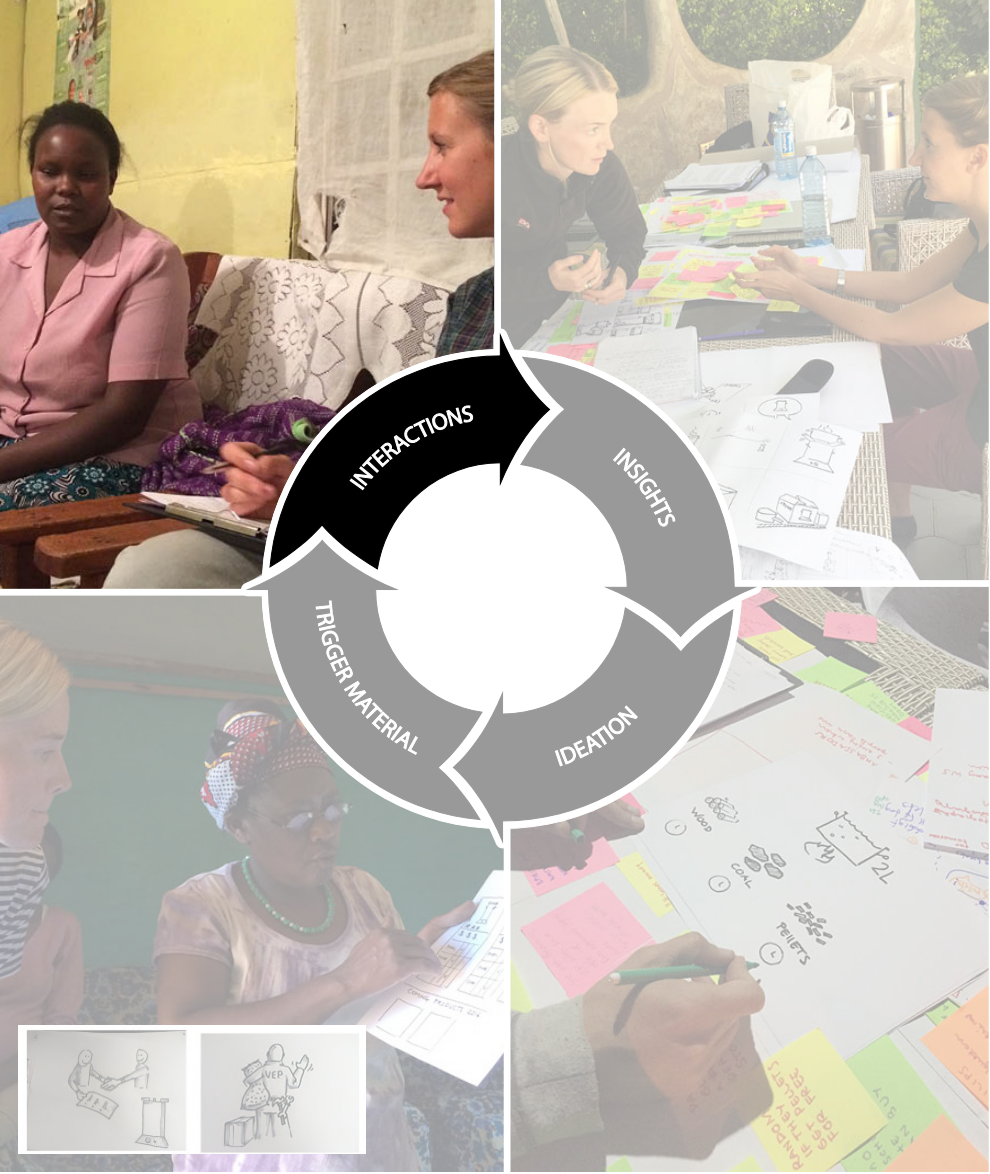
\includegraphics[width=0.7\textwidth]{Iteration.png}
    \caption{One iteration consists of Interactions, Insights, Ideation and Trigger material. The \textbf{Didactic phase} in this figure involves Insights, Ideation and Trigger material. By learning what works and not, new ideas emerge and app design is made, as well as questionnaires for evaluation. The \textbf{Technical phase} in this figure involves to code the improved app design, and evaluate how it works technically.}
    \label{fig:iteration}
\end{figure}

Each iteration ends with two check-up meetings. The first meeting is with the Experts. The next meeting is with the Partners.

The Expert group consists of Expedition Mondial and LiU Innovation. In Expert meetings, I share with them my needs. Expedition Mondial can help with the design process, and LiU Innovation can help if additional resources are needed. The meeting lasts for one hour.

The Partner group consists of most notably Iliana Björling, and preferably also Lena Tibell and Konrad Schönborn. In Partner meetings, The Analysis for the iteration is presented and discussed. Then I will propose possible decisions and discuss the alternatives. % Then I tell them about which decisions has been taken and why.
Finally, we conclude if the master thesis work is going in the right direction. These meetings should be causual and friendly, and not take a lot of time to prepare, so the next iteration can be of focus. % "Kan vara ganska vänskapligt, håll det så enkelt som möjligt så jag får tid till annat."

The time plan for the design and development phase can be seen in the section "In Uganda". The three iterations is presented below: \\

\textbf{The iterations} \\
This is how I want the process to continue:\\

	\textit{\textbf{Iteration 1}}\\
    The first iteration will have a very broad scope. The focus is on the coaches' needs, motivations, and context.  After creation of questions for questionnaire 1, I'll do interviews with coaches and other involved parties. If coaches are met in-group, open questions and dialogue will be done in group for them to be comfortable, posting anonymous answers via post-its on the wall, which leads to specific questions. These sessions will be recorded.

    %resultat: design proposal, Thoughful Interaction Design. "This is where the designer gets involved in design work, establishes a preliminary understanding of the situation, navigates through available information, and initiates all neccessary relationships with clients, users, decision makers, and so forth. Based on all this, she creates a design proposal.

    A first analysis will be done to determine needs, motivations, and expectations. Then, a summarizing meeting will be held with the expert and the partner group to determine possible ways of going forward. A first trigger/paper material will be created, for iteration 2.\\

   \textit{\textbf{Iteration 2}}\\
   This time, the iteration has a more detailed scope, with a hypothesis on what needs the app should meet and in the end, and test the trigger material created to meet those needs.

   I'll be helped with questionnaire material 2. I'll facilitate co-creating interviews with coaches, make an analysis to identify important functionality, and have a summarizing meeting with experts and partners to determine the way forward. A second trigger material will be created, one which was digital, and one which was only made on paper.\\

   \textit{\textbf{Iteration 3}}\\
   Finally, I will be supported with the third iteration, with an even more detailed scope. A co-creation workshop will be held.

   Before the workshop, the wished functionality and goals should be well formulated. Then, it can be discussed how to best design the workshop, together with Lena, Konrad, and Expedition Mondial.

   Questionnaire 3 will be created. In conjunction with the workshop the coaches can be tested, interviewed, and their interactions studied.

In the end of iteration 3, a final analysis will be done, and a final summarizing meeting with experts and partners will determine they way forward.\\


%\section{Preparations in Uganda}

\section{Iteration \#1}
Here, the work and result from iteration \#1 is presented.

\subsection*{Insights}
\textbf{Week 6-7}
Learn about the YoungDrive organization

\subsubsection{Start-up meeting with partners}
On February 10th, a first stakeholder meeting was held between me and the country managers for YoungDrive (Iliana Björling) and Plan Interational (Shifteh Malithano.

\textbf{Plan: Learn from previous work}
Led to visits and interviews with Designers without Borders and Grameen Foundation (carried out on February 26th).

Skype interview with Gerald, Plan, Tororo is used instead of both Kamuli and Tororo
Entebbe, literature review \& research
Write on the report

\subsection*{Ideation}
\textbf{Week 6}
Outbox workshop with Mango Tree
Create Workshop \#1 and Workshop \#2 with Expedition Mondial

\textbf{Week 8}
Create questionairre guide with Expedition Mondial and YoungDrive

Designers without Borders
Grameen Foundation

\subsection*{Trigger material}
Preperation
Quizical
Duolingo

\subsection*{Interactions}
\textbf{Week 7: February 23rd: Number of interactions for iteration \#1 cut down}
Interactions canceled for week 7, the day before Wednesday-Friday, because of local elections.

"Det var tråkigt att höra att det inte blev lika många interaktioner som planerat.
MEN jag tänker: Det här är verkligen en del av lärdomarna att jobba med tjänstedesign i andra kulturer (som jag även tar med mig från vårt projekt i Kenya). Det går bara att planera till en viss grad, och det blir aldrig riktigt som man tänkt sig :) Man får vara beredd på att ändra planen i sista sekund, mycket mer än vad man behöver i sin egen kultur. Bra lärdom!

Så utifrån dina fåtal interaktioner i början på nästa vecka kommer du iallafall ha en hypotes, även om den kanske är lite vagare än vad vi tänkt från början. Jag kan skicka dig nästa kapitel i Coaching Handbook som handlar om Analys senare i veckan så kan du börja fundera på hur du bäst gör analysen utifrån det material du har. " - Susanna, Expedition Mondial

\textbf{Week 7, Thursday, February 25th}
I realize what I’m actually doing is “Designing and Developing Mobile Learning for Entrepreneurship Coaches in Uganda”. The master thesis title is changed to this.

\textbf{Week 7: Friday, February 26th}
Ringer Gerald 26 fredag februari, som meddelar att nya tidschemat jag hade är omöjligt. Han har bara bokat alla inblandade kl. 8-17, då Plan inte tillåter field trips p.g.a. local elections

Krismöte med Josefina, som föreslår att gå bakom kulisserna och engagera Christine och Patrick, utan Plans inblandning. Kanske till och med kan besöka coachgrupp
Sammanfattning: interaktionerna har gått från 3 dagar, till 2 dagar, till 1 dag

Varje gång har jag behövt anpassa mig, och hitta ett nytt koncept
Nu kanske det blir 1 dag i Plans regi, och jag ändå är i Tororo måndag-onsdag.

\textbf{Week 8, Sunday-Wednesday in Tororo}
Sunday, travel to Tororo
4 (not 3 or 8) face-to-face-interviews
1 meeting with Plan, 1 with local partners
Workshop \#1: Customer Journey Map: A day as a coach
Workshop \#2: Quizical and Duolingo
2 field visits
Stay over with Patrick

\textbf{Week 8, Thursday \& Friday}
Thursday: Expert meeting with Expedition Mondial and LiU Innovation
Friday: Partner meeting with Linköping University and YoungDrive

\section{Iteration \#2}
Here, the work and result from iteration \#2 is presented.

The interactions for this iteration were planned to be in Tororo. However, during a meeting during the first week with YoungDrive project leader Josefina, I was invited to participate in the coach training in Zambia. A new work plan was created, so that I could travel to Zambia and develop the app and participate in the YoungDrive coach training together with the coaches.

\subsection*{Insights}

There were two main insights from iteration \#1.

1. The aim is for the coach to feel self-confidence for its youth session
2. The skill to be trained is having a youth session

During the evaluation meeting with Linköping University and YoungDrive, it was the determined that Iteration \#1, is answering the research question \#1, \#1a, and \#1b.

The iteration has provided a good basis for answering research question \#2.

It was concluded during the partner meeting, that iteration \#2 should:

1. Allow me to test the validity of my insights from iteration \#1.
2. Be carried out in a way that I can compare usability and learning done via the app, between iteration \#2 and \#3.

\subsection*{Ideation}

This was the start of the quiz app. The focus was on assessment. For example, it was decided with Iliana, that no facts would be presented before the quiz. 

It was discussed, how the correct information about YoungDrive would be presented. Thus, for this iteration, questions were created by the YoungDrive team, and I developed the app.

The ideation started with me creating a quide how to write questions according to Bloom's revised taxonomy, which was shared to Iliana and Josefina.

The initial plan was that the team would only produce questions for two sessions, not all 10.

Iliana did questions initially for the two sessions, mapping each question to the Bloom taxonomy.

Then, when it was decided that the app would be developed and used during an actual coach training in Zambia, it was decided that questions would be created for all sessions.

\subsection*{Trigger material}
Project leader Josefina in Zambia refined the first question sets, prepared for my visit in Zambia. Josefina created question sets with Bloom at the back of her head, also taking into account the structure and the order of the coach manuals, what it means being a coach within the topic, and lastly scenarios.

On the week before the trip, and on the airplane, I did a working prototype, a very basic quiz app, keeping it as simple as possible. I brought with be devices (tablets and smartphones).

When I arrived at the evening before the coach training started, I added the questions to the app, and installed the app to all of the devices. This process was repeated for all the days, Sunday-Friday.

\subsection*{Interactions}

\subsubsection{Design workshop \#1}
The coach training started with me having a design workshop with the coaches, not showing them the app that I had created.

Since the knowledge about smartphones and apps were low, I started by introducing these topics.

All were familiar with Facebook, so thus I showed the Facebook app. Me wanting to know what the app would look like if the coaches would have designed the app, I first needed to train them how to design an app via drawing wireframes.

Using postits, they started with during limited time drawing the start view from the Facebook app.

Then, they were asked to draw what they thought happened on the friend icon click, drawing the view on another postit.

Then, the mission of the YoungDrive app was described. They were then divided into two teams, having limited time to draw the best imaginable YoungDrive coach quiz app they could. First, they designed the app from the top of their heads. They then pitched their results to each other.

On the next iteration, they were to suggest and design improvements how the app should be designed to improve learning, not only assessment. They then again pitched their results to each other.

The result was fantastic, in the sense that it gave me an unbiased look at what the coaches expected from the app, what functionality wasn't important, and into their technical preferences.

The designs and insights gained were used throughout the week to further improve the app I had actually started creating, and gave great insights to who the coaches were and their thinking.

\subsubsection{Assessment via quiz}
At the end of each day, the app was used to test the coaches' knowledge. Each coach got either a smartphone, tablet or computer. The coach first took the quiz for the most recent session, and could then choose what to do next.

As there were no back-end developed, Josefina by hand documented the scores of each coach, writing the name of the coach, the session, number of correct answers, and what questions had been answered wrong.

Josefina then, when planning the next day, looked at the statistics, looking for trends that would inform the sessions for the following day.

She also evaluated the quality of the questions, before creating the new question sets for the next day.

\subsubsection{Experimenting with quiz before or after the session}
Since the coaches appreciated the app so much, we felt tempted to try what would happen with fun and learning if we tried using the app \textit{before} a session instead of only after. During the rest of the week, we continued, finally finding preferences and tendencies from the coaches, via observation, interviews, and survey.

\subsubsection{Experimenting with design of questions}
Number of questions
Multiple-choice questions
Framing of questions
Challenge level of questions
Determining what made a question hard

\subsubsection{Testing the app outside the YoungDrive context}
Test with refugee innovators was surprisingly successful, Humanitarian Innovation Jam
Test with university student from Makarere University scored 100\% correct

\subsection*{Result}
Using the quiz before the session increases learning, slightly decreases fun of the session

The app works for assessment!

Results from the coaches:

Trends from the coaches:

\subsection*{Analysis}
Bugs
Simpler design than I thought (KISS)

\subsection*{Discussion}
If I would have created myself, would have assumed more functionality was necessary and requested

\subsection*{Conclusion}
\begin{itemize}
\item Short iterations are very effective, however not perfect
\item Field hackathon, designing and developing together with the users, is fantastic
\item I would never have come this far without the short iterations
\item The app works for assessment!
\item Fun and encouraging and good for learning for the coaches
\item A good indicator for Josefina
\item A great way to scale the YoungDrive training in the future, both for online coach-training and the physical training
\end{itemize}


\section{Iteration \#3}

\subsection*{Insights}

Findings:
\begin{itemize}
	\item Josefina does not want to be replaced
    \item The app would be great and could actually work outside the physical coach training - with revision, be stand-alone, even being able to distribute online
    \item Refugee innovators has a great need for such an app
    \item Test with university student scored 100\% correct, means that common sense can go a long way, and that the results can't be 100\% trustworthy, and that multiple-choice questions has serious issues - this, we already knew during and before the coach training - but it needs to be taken care of
\end{itemize}

Check with findings iteration \#1:

\begin{itemize}
\item The app is only working on assessment now, not for learning
\item The need for a field app still feels relevant (especially for sessions long since the coach training)
\item The potential for YoungDrive having online coach training is huge
\end{itemize}

Determine:
\begin{itemize}
	\item Focus for the next iteration: design quiz app for learning, focus on field app (CI, CS, TM, FA), or design app that works stand-alone from the YD coach training.
\end{itemize}

\textbf{After-talk with Josefina, on Skype in Uganda, 2016-04-02:}
Nu har vi praktiska bevis för vad jag upptäckte under Iteration 1:

* Utbildningen ska faktiskt träna dem i förbereda quiz-session
* Därför borde även quiz testa detta
* Vad det inenbär vara bra coach, är hålla bra ungdomssessioner
* Det finns vissa coacher, Josefina hade velat stoppa från att hålla ungdomssession, om de inte har 90-100\% correct information
* Men hon kan inte asessa detta
* Här, är quiz en väldigt bra möjlighet
* Quiz-app under utbildning och ute i fält går därmed ihop


\subsection*{Ideation}

Josefina: “Jag kan ju inte kontrollera dem på något sätt hur de förberett sig”

Förbereda session:
Antingen inför du börjar, sedan har du ett hum vad du behöver träna mest
Eller (bättre/säkrare iom quiz inte täcker allt), så bättre förebereder sig, och sedan gör quiz när de tycker de är färdiga

Har du fått 9/10 rätt, då är du förberedd! (9-10 rätt) 
Det de har fel på, det kommer de ju lära ut ungdomarna fel på.

Om du har 8 eller under, då ligger du i röd zon
Om du har fel på t.ex. “Vad är en entreprenör?”, då kan du ju inte förklara det för ungdomarna!

Därför borde de ha alla rätt.

Där kan man ju också jobba mycket mer med feedback via appen, och skapa en annan typ av quiz för förberedande

Därför får jag Josefina att ta fram en ny quiz, som är "Förebered session X"

%https://docs.google.com/document/d/1DaVj3sOBxsnBJvQYM1UbvHcJrowaUBUnlXPYznc6csE/edit?usp=sharing 

Syftet är att komma högre upp på Bloom's revised taxonomy

Dessutom, pratade vi om utvärderings-appen: varför behöver den vara en app? Det är extremt tydligt att det fysiska ändå måste finnas. Den behövs för att ge coachen smart själv-utvärdering.

Lärdom: det passar faktiskt inom ramen för quiz-appen
Frågor blir automatiskt meta-cognitive
Passar jättebra med Learning by Reflection

\subsubsection{Monitoring \& Evaluation app can converge with Quiz App}
När någon är där och ger dem feedback, så blir det extremt svart på vitt, att de inte är så himla förberedda som de tror

Och: “Vad händer om du ger fel information här?” Vad händer om du säger cost är X?

\textbf{Varför behövs det en app för M\&E?}
För coacherna, ska få insikt på hur de håller en session
De är inte ärliga med sig själva egentligen

Appen skulle kunna ge självutvärderings-frågor?

Redan nu, så skulle man ju kunna fråga: “Vad hade hänt om du svarat X på Y?”
“Varför är det viktigt du svarar rätt på detta?”

\subsubsection{Appens fråge-struktur}

För att förbättra multiple-choice och komma högre på Bloom's taxonomy

Fyra idéer:
1. Coachernas idé från Zambia: "Gör om"-knapp (ger dig nytt quiz med bara de frågor du hade fel
2. Första idén för att lösa: håll in knapp för att spela in svar "Vad är en entreprenör?". När du klickar "Nästa", så syns multiple-choice och du väljer det alternativ som var närmast vad du svarat. Feedback experter: utmaningar med användarvänlighet (liknar Snapchat, ingen vana), du kan fortfarande välja det mest sannolika alternativet (coachen gör en självbedömning, kanske tycker A var närmast när B var närmast, och coachen kan ljuga). Fördel: YoungDrive kan använda de inspelade svaren på bra sätt. Nackdel för mig: tar tid att implementera.

3. Från Lena: gör som i NTA Digital, du får medalj guld, silver, brons baserat på hur många gånger du försökt få 100\% rätt

4. Henrik Marklund kom med följande förslag istället, inspirerat av lärare han kände: "Är du säker?" efter varje fråga
4a) Först var idén: gör som läraren, Ta fram ett gemensamt betyg, MVG, VG, G, genom att vikta Korrekthet med Empowerment
4b) Fick feedback från Josefina: ha två separata staplar Korrekthet och Empowerment. Coacherna kan 1) vilja gamea systemet, och 2) undra hur de fick sin score. Kan då bli svårt att förklara.

Fanns extremt många fördelar med denna, och kom bara fram till ännu fler efter diskussioner med människor och Lena Tibell, framför allt hur denna kan förbättra utbildningen och 1-on-1 coachning, och bli väldigt bra självreflektion för coachen.

\textbf{Sammanfattning, de 4 idéerna}

App för lärande, inte bara utvärdering.
4 vägar att gå vad gäller hur frågor ska ställas:
1. Fältmetod: Efter du har fått slutresultatet så kan du trycka på improve för att få alla felaktiga svar. Klassiskt inom körkortsproven i Sverige.

2. LiUmetod: För varje försök sänks resultaten från guld, silver och brons. Motiverar till att studera innan = gamification. 

3. Pedagogikmetod: Teknologi och förenkla livet. Efter varje fråga lades till ”hur säker är du på ditt svar?”. Kräver studenten att reflektera över sitt svar, metakognitivt tänkande.

Två staplar:
Så här mycket rätt har du / Så här empowered är du!

4. Innan du får svarsalternativen så får du spela in dina svar, sen välja ett alternativ som de tycker är närmast. Det är bra för de som utbildar coacherna.

\textbf{Beslut av approach}

Idé för interaktioner blev först att A/B-testa Idé 1+3 vs. idé 4 under en workshop, och sedan testa Idé 2 ute i fält för att mäta användbarhet, i.o.m. den metoden gav mycket kvalitativ data, och var bra feedback till utbildarna. 

Feedback kom först från Expedition Mondial (som hälsade på under veckan) att under min workshop med coacherna kommer säkert idé 1+3 och 4 blandas ihop.

Inför mitt möte med Grameen, pratade jag med innovationsrådgivare Peter Gahnström om hans analys av de 4 alternativen. Han gillade alternativ 4 mest, och gav följande nya insikt till mig: "Det här kan motverka traditioner och ”så här vi alltid gjort det” genom att tvinga en att reflektera över varför inte ens rätta svar korrelerar med hur empowered du känner dig. Bryter normer, sätter sig emot lathet och agerar proaktivt för en skarpare utveckling tillsammans."

Jag träffade Juliet och en utvecklare på Grameen Foundation (som gjort LedgerLink), och gick igenom de 4 alternativen. Svaret gavs att idé 2 definitivt är för okänd för användarna. När indikationer kom från även Grameen Foundation att 1+3 och 4 säkert skulle blandas, och var grymma alternativ, fråga jag "Hur?".

Svaret blev en diskussion med att i ett resultat efter ett quiz få två scores Korrekthet och Empowerment. Sedan på Improve, så får du medaljer/score baserat på Antal försök. (Grameen trodde ej det skulle bli problem med gamification på idé 3. ) Du ska nå t.ex. 90\% rätt på båda staplarna.

Hon (Juliet) föreslog också att du kanske inte måste ha chans på guldstjärna bara på första försöket. T.ex. att om du gör quizet gång 1, så måste du få 90\% för guld, men på ditt andra försök måste du få 95\% för guld. Detta då vi ju vill att coacherna ska ha läst på innan.

Lena Tibell menade vid förslaget att "Belöna inte hur snabbt en elev går från att kunna till att inte kunna, för olika människor lär sig olika snabbt". "Vad vi ville åstadkomma med Antal försök var endast att undvika gissningarna".

Lena frågades också om vilken skala jag ska ha på 5, 4 eller vad jag inte tänkt på, 2-gradig skala. 5 eller 4 är vilket som enligt literatur, det finns två olika skolor. 2-gradiga skalan bedömde jag vara bäst, p.g.a.
* användarvänlighet, tydligt för coacherna
* behöver inte vara krångligare än så till en början, en bra test
* blir enkelt att mäta empowerment, rätt svar + säker = pluspoäng, rätt svar + osäker = du gissade men hade rätt, gör om och var säker -> empowerment, fel svar + säker = måste ge feedback (väldigt intressant för Josefina), och fel svar + osäker = du ahde rätt, det var ett annat alternativ, gör om -> empowerment + korrekt information.

\subsubsection{Appens datainsamling}
Denna gång behövde appen samla in data av sig själv, istället för att Josefina manuellt skrev ner resultat-tavlan efter varje quiz.

Kravet kom dels från Josefina (det kommer inte gå om det är mer än 10 coacher, vi har oftast 20-30), dels från att jag i mina interaktioner i Tororo skulle testa på 2 olika kontrollgrupper med 10 personer vardera, och jag visste baserad på Interactions 1 att jag inte skulle ha tid att både skriva ner resultat och observera hur de beter sig med appen.

\textbf{Inloggning}
Att samla in data för användare, skulle kräva inloggning. Men det är ett användbarhets-problem för de flesta. Om de skapar en användare med lösenord, hur ska de 1) tycka det är intutivt och 2) komma ihåg sina användarnamn och lösenord till Interactions 4 om 2 veckor?

Jag pratade med flera om detta, Expedition Mondial och Grameen. Från EM lärde jag mig att de trodde min idé med en färdiggjort lista med coachernas namn (vi vet ju vilka som är i Tororo) skulle fungera, och från Grameen fick jag höra om dera erfarenhet att de validerat använda samma approach, med en PIN (längre än 4 siffror dock), men att de inte nailat konceptet ännu, och att de också itererar på sin approach för nästa uppdatering av LedgerLink.

Tyvärr har också Meteor begränsningar med deras auto-login-modul. Den tvingar både användarnamn och lösenord, och har automatiskt registrering. Går det att stänga av? Jag kan skapa användare och lösenord åt alla, och funderade på hur jag skulle generera lösenord. Ett förslag blev att bara registrera deras förnamn, och sedan skapa lösenordet baserat på T9 med de 6 första bokstäverna utan att berätta det för dem. Sedan tänkte jag på det kulturella, att det kan vara oartigt med förnamn, och bestämde mig för efternamn istället. Hela namnet skulle bli för långt och krångligt.

Helst skulle jag behöva gå runt Meteors standard-inloggning, och istället ha en enkel login-rullista som den ovan beskrivet, istället för att använda deras standard-lösning.

\textbf{Meteor Collections}
En annan problematik var att om data ska skickas till en server, måste det finnas en server med Collections. I version 1 av appen sparades inga resultat i huvud taget.

Jag gjorde en exempel-app med Meteor Collections under veckan, och det är ganska coolt med DDP, och appen kändes snabb oavsett ej internet-connection. Det var däremot svårt simulera samma internet-problem som ute i fält. Det är en risk jag tar, att appen kanske inte kommer skicka in rätt resultat.

Därför ville jag även ha offline-databas, och då fanns det en plugin som hette GroundDB.

Detta var tidsödande, och vi får se om det fungerar bra på måndag.

Ett annat problem är, hur ska detta visualiseras pedagogiskt för Josefina och de andra utbildarna?

\subsubsection{Educator Dashboard}
Detta hanns inte med i Iteration 3 även om det var ett mål. Istället gjordes trigger-material och workshop-upplägg till Tororo, då Expedition Mondial ifrågasatte "Visst är väl även Christine och Patrick?" målgrupp för detta? Och vad har de för utrustning? Christine har mobil, Patrick ingen. Så detta talade för att Educator Dashboard skulle behöva fungera på mobil, och inte bara dator som jag tänkt, iom att Josefina har dator.

Då bestämdes med Expedition Mondial att jag skulle ha workshop med dem på onsdag. Med samtal med Josefina, sade hon att de garanterat borde utrustas med tablets då de samlar in data digitalt, så jag kan tänka mig att de får en tablet framöver. Skönt! Detta stämmer även med vad Stefan FalkBoman hade tänkt sig, och de iPads han köpt in till mig. Så då kunde jag ha dessa som tanke att utforma educator-app-dashboarden ifrån.

\textbf{Tekniskt}

HighCharts var påtänkt som verktyg för att visualisera datan. Tanken var att den vanliga appen skulle kunna ha super-användare som är admins, och kommer till ett särskilt gränssnitt där de ser data om användarna. Detta kunde göras direkt i Meteor.

Stefan frågade vad jag tänkt om detta, och frågade om jag funderat över integration med deras verktyg Podio, och om det var möjligt. Det sade jag att det var framöver. Podio har ett API som bl.a. stödjer JSON, vilket jag använder. Då frågade jag om Podio har bra visual dash-board -verktyg, vilket han skulle kolla upp. Inom exjobbet behöver jag än så länge inte bry mig om detta. Problemet är att Stefan ser ett värde i att lagra datan i Podio, men de har inte i sig själv bra visualiseringsverktyg.

9 april hade jag då ett möte med SolarSisters COO Dave, som är en social enterprise med 1 huvudansvarig (Dave), 70 field staff och 2000 entreprenörer, så ganska likt YoungDrive i Uganda när Josefina var där.

Dave byggde 2013 upp deras backend i SalesForce för databas, och sedan TaroWorks för datainsamling. TaroWorks är en plugin till SalesForce, med offline-app anpassad för fält. De har sedan utrustat alla field staff med tablets, då det var för dyrt att ge till alla 2 000 entreprenörer. Field staff träffar entreprenörer varje dag, och hjälper entreprenörerna att knappa in t.ex. kvitton, utvärderingar och undersökningar (t.ex. från finansiärer) via appen.

Det tog 3 veckor att bara sätta upp systemet, och det var snabbt. För Dave har det varit en 100\%-tjänst i början, och fortfarande 20\%. Men fördelarna är att de nu är 100\% datadrivna, och de kan följa exakt hur det går för field staff och entreprenörerna - detta guidar även vilka som får promotions och vilka som blir avskedade.

Det mest intressanta är kanske att SolarSister inte bara avnänder datan för internt bruk, utan även för dess partners. De gör undersökningar via TaroWorks som inte är direkt kopplade till SolarSister, för att få in pengar. Men framför allt, sticker de ut gentemot andra social enterprises, då de enkelt kan ge partners all data de önskar, och det gör dem väldigt framgångsrika med grants. De är sannerligen en datadriven organisation. Datan, ger SolarSisters story ett trovärdigt narrativ, vilket Dave beskriver som en extrem framgångsfaktor.

Idag står 2/3 av finaniseringen från grants (fördel med socail entrepriser, du kan få pengar både från finansiärer och kunder), 1/3 från entreprenörerna. De vill bli mer self-sustainable för varje år som går, och detta är storyn som datan måste berätta - vilket är varför de t.ex. avskedar människor som inte presenterar. Datan måste stämma med storyn de vill berätta, för den storyn är vad som avgör att de får in pengar.

Detta gav mig insikter på hur mycket min datainsamling från coacherna kan spela roll för organisationen. Det var något jag inte tänkt på innan, och som jag vill vara medveten kring. För om det är något jag lärt mig denna iteration, är det hur "kunskap är makt", och hur mycket vettig kunskap jag, coacherna och Josefina och YoungDrive kan få ut av att helt enkelt lägga till frågan "Är du säker?" till varje quiz-fråga.

\subsubsection{Teknisk utveckling: från Meteor 1.2 till 1.3}
Branchade ut projektet och uppdaterade till Meteor 1.3 från 1.2, vilket gav bättre utvecklarupplevelse och många sådana fördelar (till exempel kan använda NPM), men fanns inte längre bakåtkompatibilitet till mobilerna som coacherna använder, samt att buildpack för Meteor till Heroku inte hade uppdaterats, så vid en push (även om det fungerade på localhost) så krashade hemsidan youngdrive.herokuapp.com, vilket fick feedback från handledare Lena som behövt accessa sidan.

Detta är ett bra exempel på hur tekniska begränsningar påverkar projektet. I slutändan, tog det ganska mycket tid under veckan "i onödan", och jag fick ta igen tiden genom att jobba fredag kväll och lördag inför mina interaktioner.

\subsection*{Trigger material}

Vad som guidade trigger material \#3, litteratur:
In particular, we theorize that, once a person has accumulated a certain amount of experience with a task, the benefit of additional practice is inferior to the benefit of reflecting upon the accumulated experience. In other words, the intentional attempt to synthesize, abstract, and articulate the key lessons learned from experience generates higher learning outcomes as compared to those generated by the accumulation of additional experience.
% https://drive.google.com/file/d/0BzlK1PD8EE75THdnRnAzWDl0VDg/view?usp=sharing
% Koppla till Bloom's Taxonomy, self-conginition

\subsection*{Interactions}

\section{Iteration \#4}

Efter prat med Henrik:
https://memorize.com/

Growht mindset vs Performance mindset
Goal-mastery-mindset vill vi få dem hamna i

Flashcards vid Improve

\textbf{Self-motitoring, vad du vill åstadkomma}
% http://digitalcommons.ilr.cornell.edu/cgi/viewcontent.cgi?article=1492&context=cahrswp

Questions Used to Prompt Self-Monitoring and Self-Evaluation
Self-Monitoring
1. Am I concentrating on learning the training material?
2. Do I have thoughts unrelated to training that interfere with my ability to focus on training?
3. Are the study tactics I have been using effective for learning the training material?
4. Am I setting learning goals to help me perform better on the final exam?
5. Am I setting learning goals to ensure that I will be ready to take the post test?
6. Have I developed a strategy for increasing my knowledge of the training material?
7. Am I setting learning goals to ensure I have a thorough understanding of the training
material?
8. Are the study strategies I'm using helping me learn the training material?
9. Am I distracted during training?
10. Am I focusing my mental effort on the training material?
Self-Evaluation
1. Do I know more about the training material than when training began?
2. Would I do better on the final exam if I studied more?
3. Do I know enough about the training material to answer at least 80% of the questions
correct on the post test?
4. Have I forgotten some of the terms introduced in previous training material?
5. Are there areas of training I am going to have a difficult time remembering for the final
exam?
6. Do I understand all of the key points of the training material?
7. Have I spent enough time reviewing to remember the information for the final exam?
8. Have I reviewed the training material as much as necessary to perform the skills on the
final exam?
9. Do I need to continue to review before taking the final exam?
10. Am I making progress towards answering at least 80% of the questions correct on the
post test? 

\subsubsection{INTERAKTIONSDESIGN FÖR LÄRANDE}
Här gås hur jag utformat appen för lärande i iteration 2 och 3 igenom, med förslag till iteration 4.

ITERATION 2

Quiz-flödet 1.0: standard multiple-choice, designat för assessment, men ej för learning
Besvara multiple-choice-frågor
Få resultat-tavla med Question 1: 0, Question 2: 1, samt "Total score: X/X"
Gå tillbaka till startskärm


ITERATION 3
Quiz-flöde 2.0: designat för learning och självreflektion, men ej för effektivitet
vid varje fråga besvarar du det alternativ du tror är rätt samt "Are you sure?" Yes/No
vid färdigt quiz, få en resultattavla med personliserad feedback
läsa igenom dina felaktiga svar och hur säker du varit på dem 
observerat de korrekta svaren
klicka "Improve" för att bara få dina felaktiga svar igen
upprepa tills inga felaktiga svar var kvar (det står "quiz try: 3", om det är försök 3)
vid 100%, låsa upp "I can get 100%" (som är hela quizet igen)
innan dess, uppmuntrades du läsa igenom coach/deltagar-manualen
om du då fick något fel, fick du gå tillbaka till träning igen
om alla rätt på, blev du Certified coach. Om du klarade det på första försöket, fick du även en guldstjärna (andra försöket = silver, tredje försöket = brons)
sedan kunde du ta ett annat quiz
Kommentar, fördelar med feedback-läge:
Genom att på varje fråga besvara "Are you sure?": Yes/No, så stärker vi inte bara coachens meta-kognitiva förmåga, utan vi kan vi även ge personliserad feedback i resultattavlan, istället för att bara visa Question 1: 1 point. Question 2: 0 points, som i Iteration 2.

Detta gör att coachen kan reflektera över sitt lärande på t.ex. följande sätt:
- få en självförtroende-boost (via feedback "You were correct, and you were sure")
- gå från gissning till självsäkerhet (via feedback "You guessed, but you were correct")
- ändra uppfattning snabbare (via feedback "You were incorrect, but you were sure")
- uppmuntra coachen att läsa i manualen (via feedback "You were incorrect, and you were not sure")

Fördelar med tränings-läge, och certifikations-läge:
Jag gillar idén att när coachen har kunnat svara rätt på alla frågor, kunna befästa kunskapen med hjälp av certifikations-läget, då coachen ska kunna få 100% rätt på 1 försök.

FÖRSLAG ITERATION 4: designat för learning och självreflektion, och effektivitet
Problemet nu, var att de tog certifikations-läget och inte fick 100%, vilket är mödosamt och väldigt tidsslösande, då coachen igen måste gå tillbaka till Träning och nå 100% igen. 

Tränings-läget behöver alltså förbättras, och vara säker på att coachen verkligen är redo för Certification. 

Ett problem är att "Improve" endast upprepade frågor som varit inkorrekta, och inte upprepade gissningar som varit rätt. Det gjorde att en coach kunde få fel på Certification quiz, för att kunskapen inte var befäst. Så vill vi inte ha det. Därför föreslår jag följande förbättringar i Träningsläge:

Förbättringar Träningsläge: ta ett quiz, med "Are you sure?". Baserat på svar, låt frågor hamna i tre olika lådor: "Can't do", "Can do with effort" och "Can do effortlessly".

Låt coachen välja vilken typ av frågor de vill upprepa. 

Frågor i "Can't do", är frågor som coachen ej vet svar på ännu (t.ex. om svarat fel). 
Frågor i "Can do with effort", har coachen ett hum om (gissat rätt, eller gått från fel till rätt). 
Frågor i "Can do effortlessly", har coachen rätt och den vet att den har rätt

Genom att ta en hög med frågor igen, flyttas de om till andra högar. Om du har fel på en "Can do effortlessly"-fråga, flyttas den tilllbaka till "Can't do" eller "Can do with effort". Om coachen igen har rätt på en "Can do effortlessly", blir coachen certified i just den frågan.

Frågor i "Certified", är frågor som coachen befäst genom att upprepat korrekt från "Can do effortlessly". De behöver inte upprepas. Coachen kan bli Certified i ett helt quiz, när den tar alla frågor som ligger i Certified. Då är den klar, och 100% expert i ämnet! Men coachen kan också välja att lämna quizet när som helst, och komma tillbaka i ett senare tillfälle. Detta handlar om glädjen i att lära sig, bli en bättre coach, och att visuellt se hur man blir bättre hela tiden.

Målet är alltså att i coachens egna tempo, flytta över frågor från "Can't do" till "Can do effortlessly" till "Certified". Så planerar jag bygga expertis som YoungDrive-coach.

Förbättringar Certifikationsläge: om coachen klarar det, ska coachen bli enormt glad. Guld, silver och brons-medaljer ska vara tydliga, och ljud kan förstärka storheten i att ha klarat det. Det ska synas på startskärmen, att du har fått stjärnor och blivit certifierad i ett topic.

\subsubsection{Service design-insikter}

SERVICE DESIGN
Detta kapitel visar vilka insikter som har guidat mitt arbete med iteration 1, 2, 3 och 4.

ITERATION 1 \& 3: What's it like being a coach? 
I iteration 1 fanns ingen digital ansats alls. Jag var i Tororo för att besvara "What's it like being a coach?". Upptäckte att vad det innebär att vara en bra YoungDrive-coach, är att kunna ha bra ungdoms-sessioner. För att ha bra ungdoms-sessioner, är din självkänsla och självförtroende enormt viktigt. Och det är inte alla coacher som har detta, och därför skiljer sig kvaliteten mycket, vilket Josefina upplever som en utmaning.

Jag började leta efter hur och var en coach-app kan underlätta. En aktivitet som alla coacher har gemensamt för lärande och avgörande för coachens framgång, är (1) coach-träningen (som jag redan visste var viktig), men framför allt (2) förberedelserna av en ungdomssession. Jag övertygade Josefina att vi skulle ha ett mycket fokus på (2) än hon tänkt. Medan Josefina kan vara inblandad i (1), kan en app vara extremt viktig i (2), upptäckte jag under mina fält-besök på ungdomssessioner och intervjuer med coacher och projektledare.

I Tororo iteration 1 kunde jag observera ungdomsbesöken, i Zambia iteration 2 kunde jag observera coach-träningen, och i iteration 3 i Tororo kunde jag observera förberedande av ungdoms-sessioner.

Därför fick app-utvecklingen för dessa iterationer ha dessa fokus. I iteration 1 fanns ingen digital ansats, men apparna Quizical och Duolingo testades för att få koll på coachernas tekniska förutsättningar. Resultatet blev att min app kan placera sig någonstans emellan i svårighetsgrad.

Iteration 2 gjordes en coach assessment quiz app, och iteration 3 utvecklades den till en coach learning quiz app. Dessa insikter guidade:

Iteration 1: Självförtroende = empowerment
Enligt iteration 1 kom självförtroende ifrån att under ungdomstillfället kunna ha: Correct Information, Correct Structure, Time Management, och Fun Atmosphere. Det är alltså detta appen borde testa och träna.

Lösning: en coach-träningss-app hade störst behov av att fokusera på Correct Information, i andra hand Correct Structure och Time Management. Till iteration 2 kunde Josefina assessa Correct Information (lyckat), och till iteration 3 kunde coacherna lära sig CI (lyckat, men behöver göras mer effektivt). Till iteration 3 hade hon via ett "Are you ready?"-quiz även försökt använda multiple-choice-strukturen till att även assessa och träna Correct Structure och Time Management (ej särskilt effektivt sätt, testar Factual Remember, men ej högre Bloom). 

Det finns en medvetenhet kring att CS, TM och Fun Atmosphere är lämpligast att testa efter en ungdomssession, men att vissa förberedelser kan göras i appen innan en session. Dessa är därför sekundära.

Iteration 2 och 3: Självkänsla = kunskap om dig själv, meta-kognition
Under Iteration 2 i Zambia, passade jag på att fråga vad som byggde självkänsla. Följande kluster fanns: "I believe in myself" (3 personer), "I believe in God" (2 personer), men också "I am well prepared" (4 personer) och "I am certified" (1 person).

Till iteration 2, hade jag fokuserat på att assessa "I am well prepared" och då stärka självförtroende, med hänsyn till Correct Information. 

I iteration 3 i Tororo, hade jag fokuserat på att bli "I am well prepared", och även byggt in "I am certified.". Det visar sig att de flesta inte bryr sig om "I am certified" (vilket ju undersökningen redan visade), men de bryr sig om lärande-resultaten.

Under iteration 3, lärde jag mig att det tog för lång tid för coacher att nå 100% säkerhet. Detta blev tydligt särskilt på den svåraste quizen om Correct Structure och Time Management, "Week 9: Are you ready?", då det tog en coach 2.5 timme att nå 100% i ett försök. I iteration 2, då "Improve" inte fanns, hade detta nog tagit ännu längre tid.

Iteration 4: Effektivitet = en förutsättning för att coacherna ska ha nytta av appen
Anledningen till misslyckandet i iteration 3: dels för att CS och TM tydligen inte lämpar sig för multiple-choice (gör sådana övningar drag-and-drop-istället), men framför allt för att feedback-systemet och tränings-läget behöver vara mer medvetet i när en coach verkligen kan sitt ämne och är redo för sin ungdomssession. Du vill inte testa 100% rätt utan fel på 13 frågor, förrän du är helt säker på att en coach är färdig med sin träning. Till iteration 4, vill jag göra appen effektiv.

